\section{Advanced Techniques}

	\subsection{Step-by-step pattern}

		The Step-by-step pattern was used previously in the book.
		It is very useful to use it for observation purposes, that is, to observe how a fractal evolves over time.
		
	    Suppose that Layer 1 has a simple transformation, for example the Koch Snowflake.
	    Then suppose that Layer 2 has the following transformation (fig.\ref{step_01}).

	    \begin{figure}[H]
	    	\centering
	    	\caption{\label{step_01} Step-by-step pattern.}
	    	\subcaptionbox{Koch Snowflake.}[0.3\TW]
                {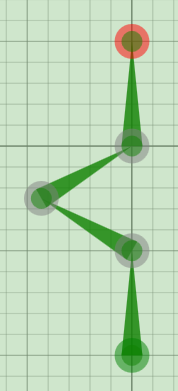
\includegraphics[height=0.3\TW]{img/Advanced_Techniques/Step/step_set_02.png}}
            ~
            \subcaptionbox{Step-by-step pattern.}[0.3\TW]
                {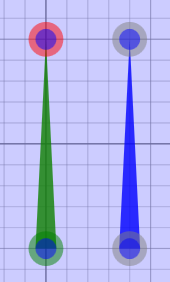
\includegraphics[height=0.3\TW]{img/Advanced_Techniques/Step/step_set_01.png}}
	    \end{figure}

	    \begin{figure}[H]
	    	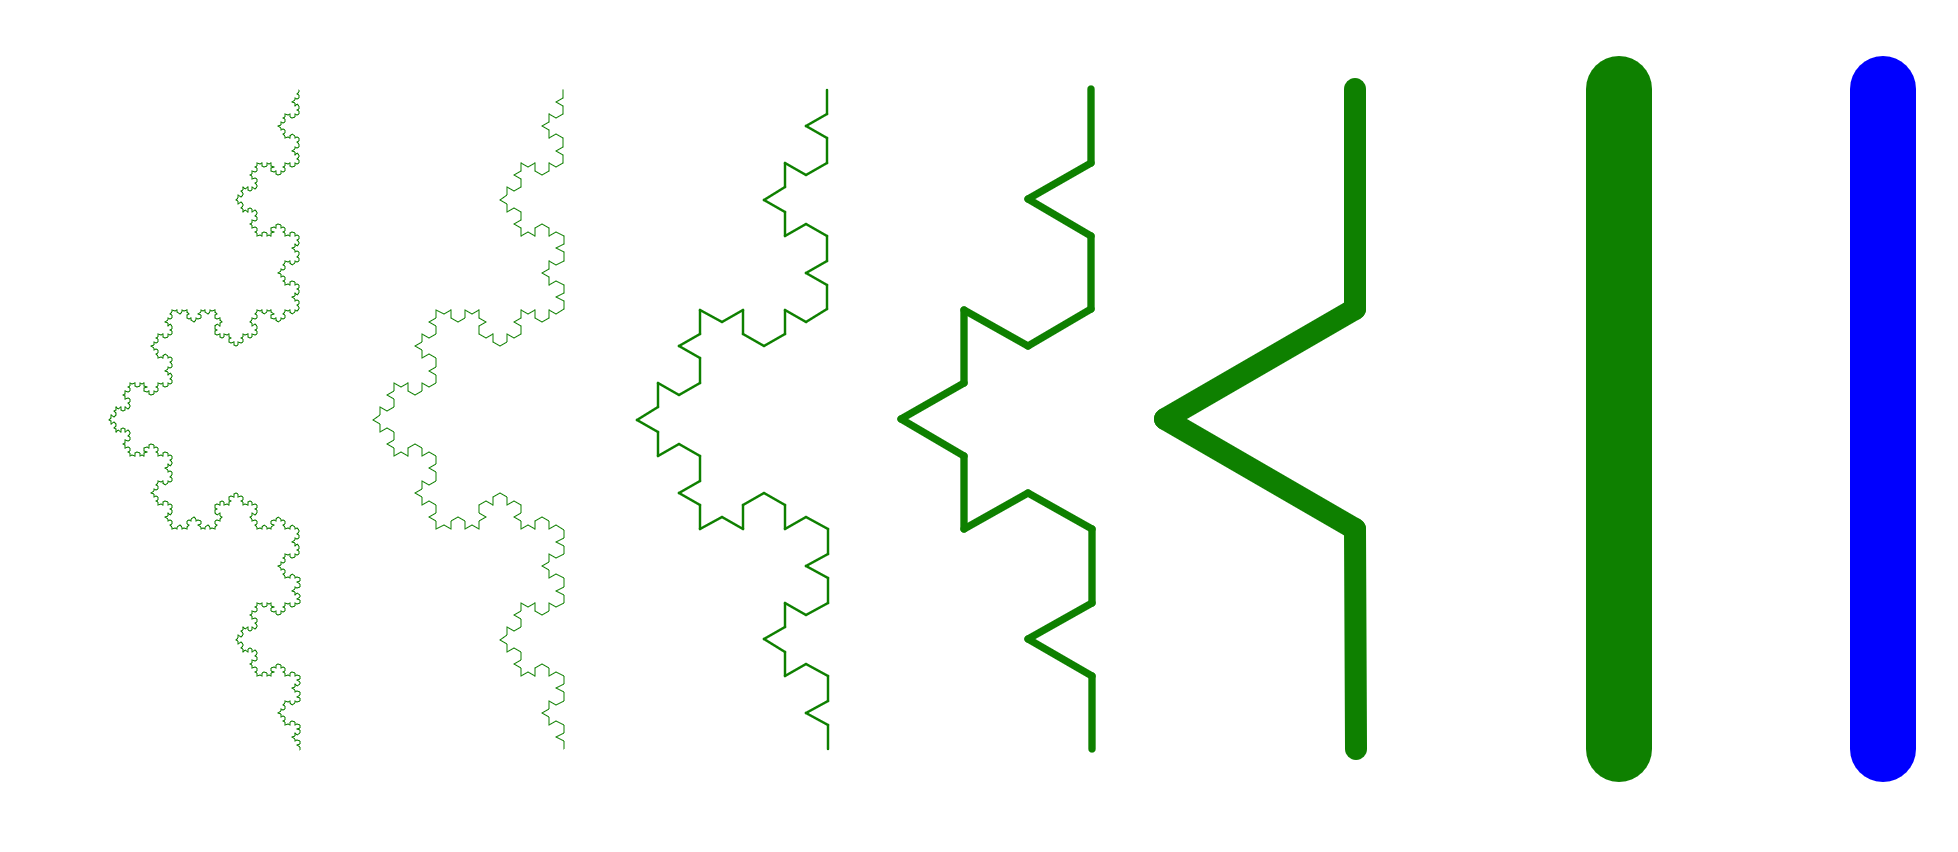
\includegraphics[width=0.9\TW]{img/Advanced_Techniques/Step/step_01.png}
	    \end{figure}

	    Layer 2 works by creating a desired iteration and then calling himself a little further.
	    In this way the development of the fractal becomes very clear.
	    Of course it is not necessary that the segments in the Step-by-step transformation should be parallel to each other.
	    We can choose a circular configuration.
	    The blue color can be removed by pressing the X in color-choosing dialog.

	    \begin{figure}[H]
	    	\centering
	    	\caption{\label{step_03} Step-by-step pattern.}
	    	\subcaptionbox{The setup.}[0.25\TW]
                {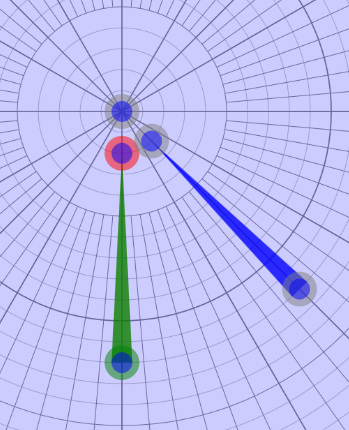
\includegraphics[width=0.25\TW]{img/Advanced_Techniques/Step/step_set_03.png}}
            ~
            \subcaptionbox{The fractal.}[0.5\TW]
                {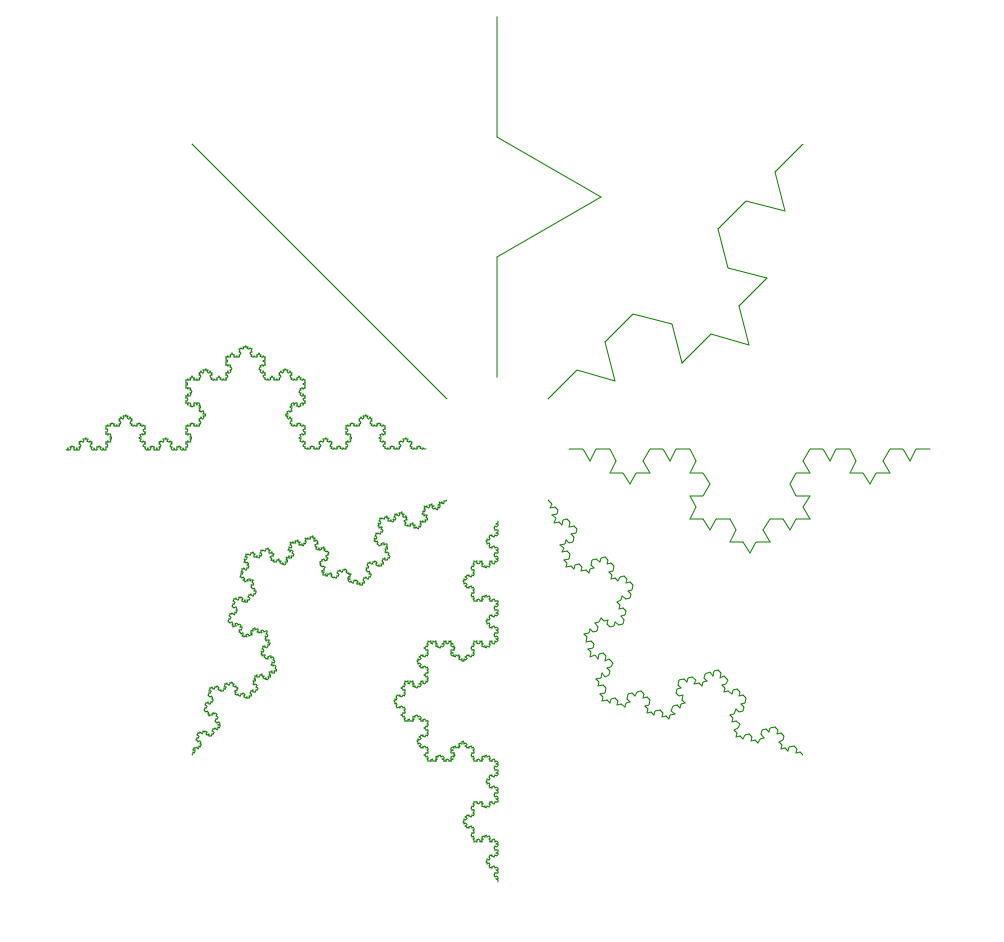
\includegraphics[width=0.5\TW]{img/Advanced_Techniques/Step/step_03.png}}
	    \end{figure}

	\subsection{Color Mixing}

		This is more of a trick than a relevant mathematical concept.
		While a complex figure is being drawn, the user can choose a different color for the segments.
		Figure~\ref{mix_01} shows this technique applied to the dragon curve.

		\begin{figure}[H]
			\centering
			\caption{\label{mix_01} Colored Dragon}
	    	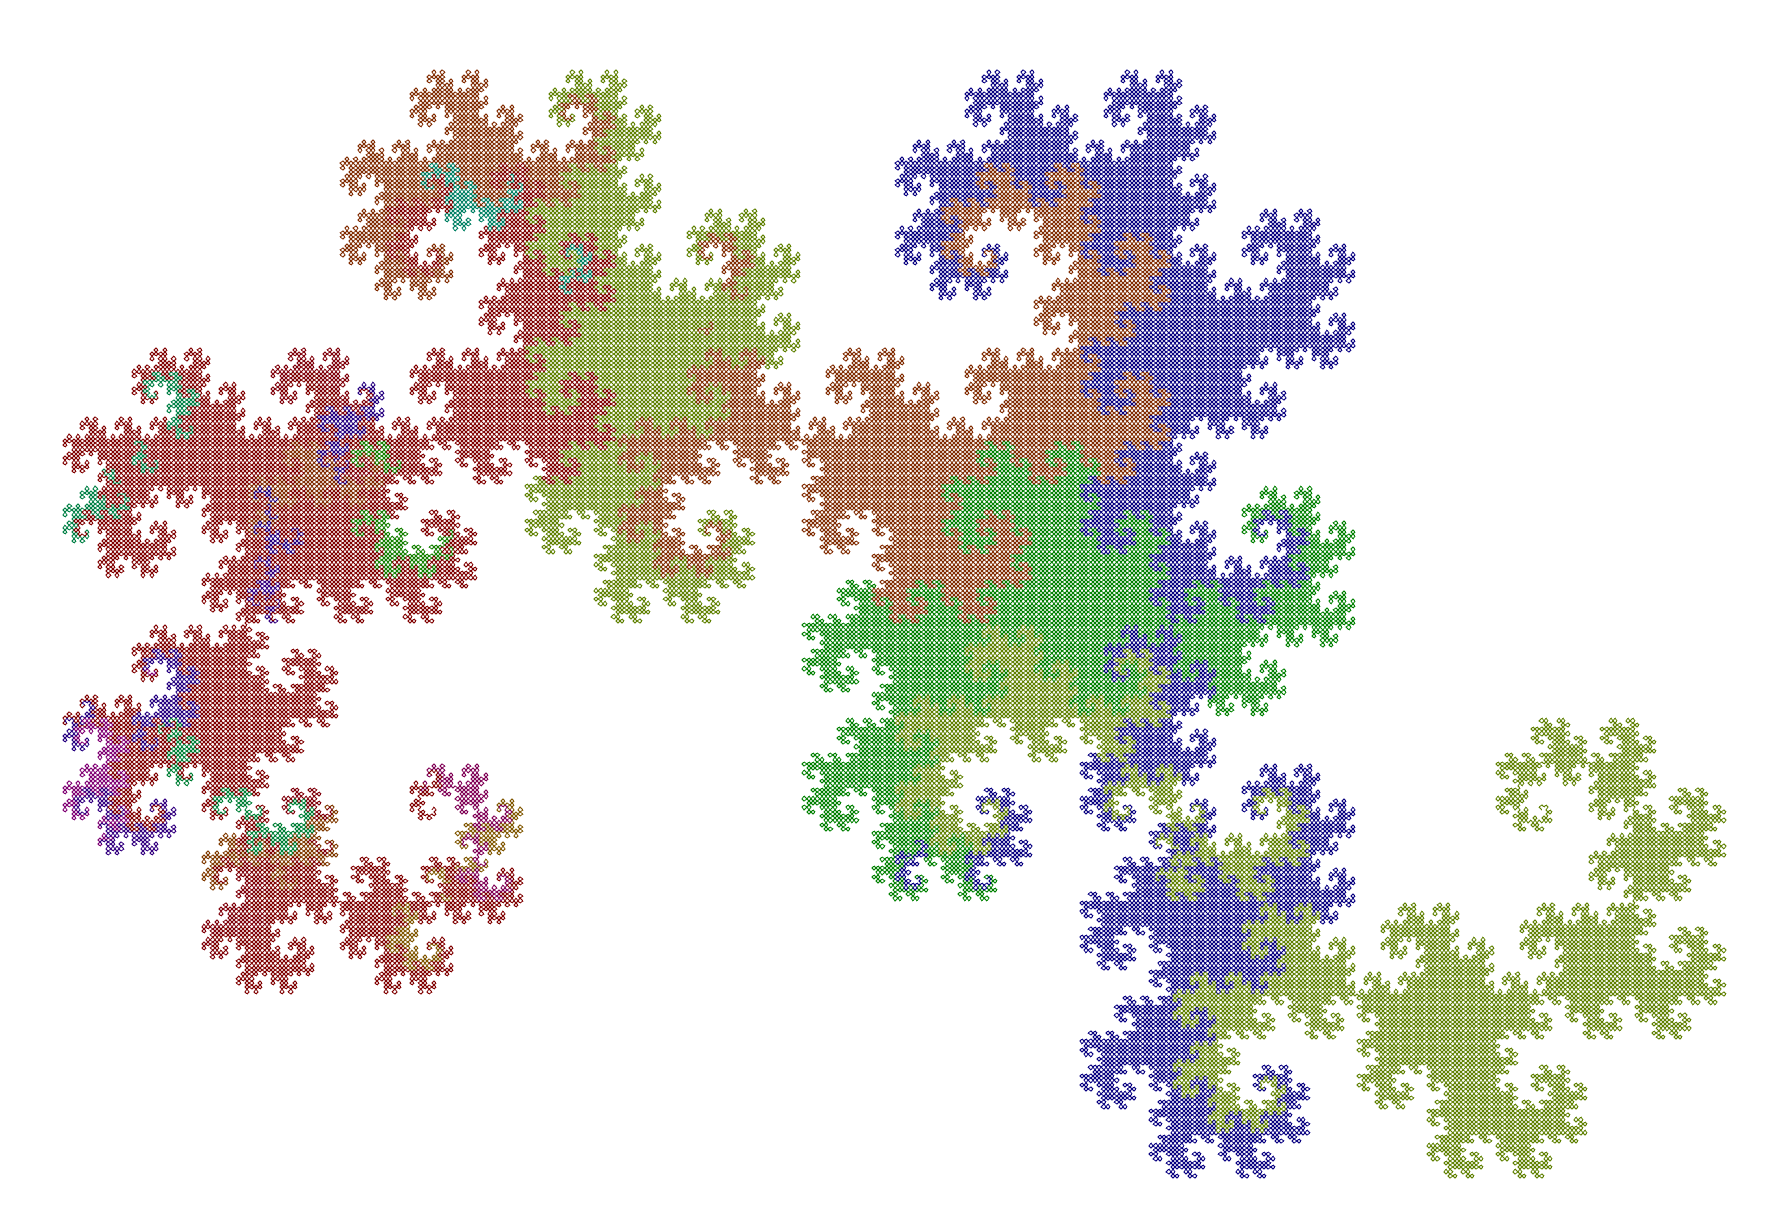
\includegraphics[width=0.8\TW]{img/Advanced_Techniques/Mixing/mix_01.png}
	    \end{figure}